\section{El Grupo Fundamental}
\indicetema{t3}

\subsection{Arcos, lazos y homotopía relativa}

Sea $X$ e.t., $x_0, x_1 \in X$. Al conjunto $C_{x_0, x_1}(X) = \{ \alpha \colon [0,1] \to X \text{ cont } \mid \alpha(0) = x_0, \alpha(1) = x_1 \}$ se le denomina conjunto de arcos o caminos. 

Saber que dos arcos cualesquiera son homotópicos no es suficiente para "cazar" agujeros topológicos. Por ello, requerimos fijar subconjuntos durante la deformación.

\begin{definicion}{Homotopía relativa [C3.7]}{def_homotopia_relativa}
Sea $A \subseteq X$. Sean $f, g \colon X \to Y$ continuas. Diremos que $f, g$ son homotópicas respecto a $A$ (denotado $f \simeq_A g$) cuando $\exists F \colon X \times I \to Y$ continua tal que:
\begin{enumerate}
    \item $F_0 = f$
    \item $F_1 = g$
    \item $\forall a \in A, \forall t \in I \colon F(a,t)$ es constante (no depende de $t$). En particular, $F(a,t) = f(a) = g(a) \ \forall t \in I$.
\end{enumerate}
\end{definicion}

Para caminos con extremos fijos, $\alpha \simeq_{\{0,1\}} \beta \iff \exists F \colon I \times I \to X$ continua tal que:
1. $F_0 = \alpha$ \\
2. $F_1 = \beta$ \\
3. $F(0,t) = \alpha(0) = \beta(0)$, y $F(1,t) = \alpha(1) = \beta(1) \quad \forall t \in I$.

Si $x_0 = x_1$, notaremos $C_{x_0}(X)$ al conjunto de \textbf{lazos} con base en $x_0$.

\begin{observacion}{Propiedades de la homotopía relativa [C3.8]}{obs_relativa}
\begin{enumerate}
    \item Si $f \simeq_A g$ mediante $F$, entonces para cada $a \in A$ se tiene $F_t(a) = F(a,t) = f(a)$ para todo $t \in I$. En particular $F_t(A) = f(A)$ no depende de $t$: $A$ permanece invariante (de hecho, punto a punto) durante la deformación.
    \item En consecuencia, $f \simeq_A g \implies f|_A = g|_A$. Solo pueden ser homotópicas relativas a $A$ aplicaciones que coinciden sobre $A$.
    \item Si $f \simeq_A g$ entonces $f \simeq g$, pero el recíproco es falso: $\simeq_{\{0,1\}}$ es mucho más restrictiva que $\simeq$. Por ejemplo, si $X$ es arco-conexo, \emph{cualesquiera} dos aplicaciones $\alpha, \beta \colon I \to X$ son homotópicas: $F(s,t) = \alpha((1-t)s)$ da $\alpha \simeq c_{\alpha(0)}$, y si $\gamma$ es un arco de $\alpha(0)$ a $\beta(0)$, $H(s,t) = \gamma(t)$ da $c_{\alpha(0)} \simeq c_{\beta(0)} \simeq \beta$. En cambio, en $S^1$ el lazo constante $c_1$ y el lazo $s \mapsto e^{2\pi i s}$ \emph{no} son homotópicos relativos a $\{0,1\}$ (veremos que $\pi_1(S^1) \cong \mathbb{Z}$). Es esta rigidez la que permite ``cazar agujeros''.
\end{enumerate}
\end{observacion}

\begin{teorema}{Relación de equivalencia relativa [C3.9] \marcaT \marcaE}{teo_rbe_relativa}
La relación $\simeq_A$ es una R.B.E. en $C(X,Y)$. 
\end{teorema}

\begin{proof}
Es la misma prueba que para $\simeq$, comprobando además que $A$ queda fijo.
\begin{enumerate}
    \item \textbf{Reflexiva:} $F(x,t) = f(x)$ cumple $F_0 = F_1 = f$ y $F(a,t) = f(a)$ para todo $a \in A$.
    \item \textbf{Simétrica:} si $F \colon f \simeq_A g$, definimos $G(x,t) = F(x,1-t)$. Entonces $G_0 = g$, $G_1 = f$ y $G(a,t) = F(a,1-t) = f(a) = g(a)$ no depende de $t$.
    \item \textbf{Transitiva:} sean $F^{(1)} \colon f \simeq_A g$ y $F^{(2)} \colon g \simeq_A h$. Definimos $F(x,t) = F^{(1)}(x,2t)$ si $t \in [0,\frac12]$ y $F(x,t) = F^{(2)}(x,2t-1)$ si $t \in [\frac12,1]$, que es continua como en el \cref{thm:teo_rel_eq}. Para $a \in A$: si $t \le \frac12$, $F(a,t) = f(a)$; si $t \ge \frac12$, $F(a,t) = g(a) = f(a)$ (porque $f|_A = g|_A$ por la observación anterior). Luego $F(a,t)$ es constante en $t$ y $f \simeq_A h$.
\end{enumerate}
\end{proof}

\subsection{El grupo fundamental y el teorema de Poincaré}

\begin{definicion}{Grupo fundamental [C3.17]}{def_grupo_fundamental}
Sea $X$ e.t., sea $x_0 \in X$. Definimos el grupo fundamental de $X$ en $x_0$, denotado como $\pi_1(X, x_0)$, al conjunto cociente de lazos bajo homotopía relativa a los extremos:
\[ \pi_1(X, x_0) \equiv C_{x_0}(X) / \simeq_{\{0,1\}} \]
A la clase de equivalencia de un lazo $\alpha$ la denotamos como $[\alpha]$.

Es importante notar que aun no hemos demostrado que se trata de un grupo, se demuestra en \cref{thm:poincare}
\end{definicion}

Para dotar a $\pi_1(X, x_0)$ de estructura de grupo, introducimos operaciones en caminos:
Sean $x_0, x_1, x_2 \in X$ y caminos $\alpha \colon I \to X$ (de $x_0$ a $x_1$) y $\beta \colon I \to X$ (de $x_1$ a $x_2$).
Definimos la \textbf{concatenación} $\gamma = \alpha * \beta \colon I \to X$ dada por:
\[ \gamma(t) = \begin{cases} \alpha(2t), & \forall t \in [0, 1/2] \\ \beta(2t-1), & \forall t \in [1/2, 1] \end{cases} \]
Definimos el \textbf{camino inverso} $\alpha^{-1} \colon I \to X$ como $\alpha^{-1}(t) = \alpha(1-t)$, el cual va de $x_1$ a $x_0$.

\begin{teorema}{Conexión por caminos [C3.6] \marcaT}{teo_contractil_arcoconexo}
Sea $X$ contractil. Entonces $X$ es arco-conexo.
\end{teorema}
\begin{proof}
Sean $x, y \in X$. Por ser contractil, $\exists x_0 \in X \mid 1_X \simeq c_{x_0}$. Es decir, $\exists F \colon X \times I \to X$ continua con $F_0 = 1_X, F_1 = c_{x_0}$.
Definimos el camino $\alpha \colon I \to X$ dado por $t \mapsto F(x,t)$, que une $\alpha(0)=x$ con $\alpha(1)=x_0$.
Definimos el camino $\beta \colon I \to X$ dado por $t \mapsto F(y,t)$, que une $\beta(0)=y$ con $\beta(1)=x_0$.
El camino concatenado $\delta = \alpha * \beta^{-1}$ une los puntos $x$ e $y$ de forma continua.
\end{proof}

\begin{observacion}{El recíproco es falso [C3.6]}{obs_recip_contractil}
Arco-conexo $\not\implies$ contráctil. El ejemplo es $S^1$: es arco-conexo, pero no es contráctil, pues veremos que $\pi_1(S^1) \cong \mathbb{Z} \neq 1$, mientras que todo espacio contráctil tiene grupo fundamental trivial.
\end{observacion}

\begin{nota}{Asociatividad de caminos [C3.13]}{nota_asociatividad}
Es importante notar que $\alpha * (\beta * \gamma) \neq (\alpha * \beta) * \gamma$ a nivel de aplicaciones, ya que las parametrizaciones difieren en los intervalos temporales. Sin embargo, sí son equivalentes bajo homotopía relativa a los extremos. 
Definimos entonces el producto de clases como:
\[ [\alpha] \cdot [\beta] = [\alpha * \beta] \]
\end{nota}

\begin{teorema}{de Poincaré [C3.16] \marcaT}{poincare}
Sea $X$ un espacio topológico y sea $x_0 \in X$. Entonces 
\[
(\pi_1(X, x_0), \cdot)
\]
es un grupo.
\end{teorema}

\textbf{18/09/2026}

\begin{proof}
Dividimos la demostración en la comprobación de la buena definición de la operación y el cumplimiento de los axiomas de grupo:

\begin{enumerate}
    \item \textbf{La operación está bien definida.}
    
    Sean $\alpha, \alpha', \beta, \beta' \in \mathcal{C}_{x_0}(X)$. Se debe probar que:
    \[
    \left.
    \begin{aligned}
    \alpha &\simeq_{\{0,1\}} \alpha' \\
    \beta &\simeq_{\{0,1\}} \beta'
    \end{aligned}
    \right\} \implies \alpha * \beta \simeq_{\{0,1\}} \alpha' * \beta'
    \]
    Por hipótesis, existen homotopías relativas:
    \begin{itemize}
        \item $H^{(1)} : I \times I \to X$ continua con:
        \[
        H_0^{(1)} = \alpha, \quad H_1^{(1)} = \alpha', \quad H^{(1)}(0, t) = \alpha(0) = \alpha'(0) = x_0, \quad H^{(1)}(1, t) = \alpha(1) = \alpha'(1) = x_0 \quad (\forall t \in I)
        \]
        \item $H^{(2)} : I \times I \to X$ continua con:
        \[
        H_0^{(2)} = \beta, \quad H_1^{(2)} = \beta', \quad H^{(2)}(0, t) = x_0, \quad H^{(2)}(1, t) = x_0 \quad (\forall t \in I)
        \]
    \end{itemize}

    Se define la aplicación $H : I \times I \to X$ dada a trozos por:
    \[
    H(s, t) = 
    \begin{cases}
    H^{(1)}(2s, t) & \text{si } s \in [0, 1/2], \\
    H^{(2)}(2s - 1, t) & \text{si } s \in [1/2, 1].
    \end{cases}
    \]

    \begin{itemize}
        \item \emph{Coincidencia en la frontera común ($s = 1/2$):}
        \[
        H(1/2, t) = 
        \begin{cases}
        H^{(1)}\left(2 \cdot \frac{1}{2}, t\right) = H^{(1)}(1, t) = x_0, \\
        H^{(2)}\left(2 \cdot \frac{1}{2} - 1, t\right) = H^{(2)}(0, t) = x_0.
        \end{cases}
        \]
        Por tanto, $H$ está bien definida.

        \item \emph{Continuidad de $H$:}
        Escribimos $I \times I = B_1 \cup B_2$, donde:
        \[
        B_1 = [0, 1/2] \times I, \qquad B_2 = [1/2, 1] \times I
        \]
        Ambos subconjuntos son cerrados en $I \times I$. Como $H|_{B_1}$ y $H|_{B_2}$ son continuas y coinciden en $B_1 \cap B_2$, por el lema de pegamiento (continuidad a trozos), $H$ es continua.

        \item \emph{Instantes $t = 0$ y $t = 1$:}
        \[
        H_0(s) = H(s, 0) = 
        \begin{cases}
        H^{(1)}(2s, 0) = \alpha(2s) & \text{si } s \in [0, 1/2], \\
        H^{(2)}(2s - 1, 0) = \beta(2s - 1) & \text{si } s \in [1/2, 1],
        \end{cases}
        \implies H_0 = \alpha * \beta
        \]
        \[
        H_1(s) = H(s, 1) = 
        \begin{cases}
        H^{(1)}(2s, 1) = \alpha'(2s) & \text{si } s \in [0, 1/2], \\
        H^{(2)}(2s - 1, 1) = \beta'(2s - 1) & \text{si } s \in [1/2, 1],
        \end{cases}
        \implies H_1 = \alpha' * \beta'
        \]

        \item \emph{Fijación de los extremos ($s = 0$ y $s = 1$):}
        \[
        \begin{aligned}
        H(0, t) &= H^{(1)}(0, t) = x_0, \\
        H(1, t) &= H^{(2)}(1, t) = x_0.
        \end{aligned}
        \]
        No dependen de $t$. En consecuencia, $H : \alpha * \beta \simeq_{\{0,1\}} \alpha' * \beta'$.
    \end{itemize}

    \item \textbf{Propiedad asociativa.}
    
    Se debe probar que:
    \[
    [\alpha] \cdot ([\beta] \cdot [\gamma]) = ([\alpha] \cdot [\beta]) \cdot [\gamma], \quad \forall \alpha, \beta, \gamma \in \mathcal{C}_{x_0}(X)
    \]
    lo cual equivale a demostrar que $(\alpha * \beta) * \gamma \simeq_{\{0,1\}} \alpha * (\beta * \gamma)$.
    
    Explícitamente, las parametrizaciones son:
    \[
    ((\alpha * \beta) * \gamma)(s) = 
    \begin{cases}
    \alpha(4s) & \text{si } s \in [0, 1/4], \\
    \beta(4s - 1) & \text{si } s \in [1/4, 1/2], \\
    \gamma(2s - 1) & \text{si } s \in [1/2, 1];
    \end{cases}
    \]
    \[
    (\alpha * (\beta * \gamma))(s) = 
    \begin{cases}
    \alpha(2s) & \text{si } s \in [0, 1/2], \\
    \beta(4s - 2) & \text{si } s \in [1/2, 3/4], \\
    \gamma(4s - 3) & \text{si } s \in [3/4, 1].
    \end{cases}
    \]
    
    Se define la homotopía $H : I \times I \to X$ mediante reparametrizaciones afines a trozos sobre los intervalos que varían linealmente con $t$:
    \[
    H(s, t) = 
    \begin{cases}
    \alpha\left( \dfrac{4}{t + 1} s \right) & \text{si } s \in \left[ 0, \dfrac{t+1}{4} \right], \\[2ex]
    \beta(4s - t - 1) & \text{si } s \in \left[ \dfrac{t+1}{4}, \dfrac{t+2}{4} \right], \\[2ex]
    \gamma\left( \dfrac{4s - 2 - t}{2 - t} \right) & \text{si } s \in \left[ \dfrac{t+2}{4}, 1 \right].
    \end{cases}
    \]
    
    \begin{itemize}
        \item \emph{Buena definición en las fronteras:}
        \begin{itemize}
            \item En $s = \frac{t+1}{4}$:
            \[
            \alpha\left( \frac{4}{t+1} \cdot \frac{t+1}{4} \right) = \alpha(1) = x_0, \qquad \beta\left( 4 \cdot \frac{t+1}{4} - t - 1 \right) = \beta(0) = x_0.
            \]
            \item En $s = \frac{t+2}{4}$:
            \[
            \beta\left( 4 \cdot \frac{t+2}{4} - t - 1 \right) = \beta(1) = x_0, \qquad \gamma\left( \frac{4\frac{t+2}{4} - 2 - t}{2 - t} \right) = \gamma(0) = x_0.
            \]
        \end{itemize}
        \item \emph{Continuidad:} Por el lema de pegamiento en los subconjuntos cerrados determinados por las rectas $s = \frac{t+1}{4}$ y $s = \frac{t+2}{4}$, $H$ es continua.
        \item \emph{Evaluación en los extremos temporales:}
        \[
        H(s, 0) = ((\alpha * \beta) * \gamma)(s), \qquad H(s, 1) = (\alpha * (\beta * \gamma))(s).
        \]
        \item \emph{Extremos espaciales:}
        \[
        H(0, t) = \alpha(0) = x_0, \qquad H(1, t) = \gamma(1) = x_0 \quad (\forall t \in I).
        \]
    \end{itemize}
    Por tanto, $H$ es una homotopía relativa y la operación es asociativa.

    \item \textbf{Existencia de elemento neutro.}
    
    Sea $c_{x_0} : I \to X$ el lazo constante $c_{x_0}(s) = x_0$ para todo $s \in I$. Se debe probar que:
    \[
    [c_{x_0}] \cdot [\alpha] = [\alpha] \iff c_{x_0} * \alpha \simeq_{\{0,1\}} \alpha.
    \]
    El producto con el neutro es:
    \[
    (c_{x_0} * \alpha)(s) = 
    \begin{cases}
    c_{x_0}(2s) = x_0 & \text{si } s \in [0, 1/2], \\
    \alpha(2s - 1) & \text{si } s \in [1/2, 1].
    \end{cases}
    \]
    Se construye la homotopía $F : I \times I \to X$:
    \[
    F(s, t) = 
    \begin{cases}
    x_0 & \text{si } s \in \left[0, \dfrac{1-t}{2}\right], \\[2ex]
    \alpha\left( \dfrac{2s + t - 1}{t + 1} \right) & \text{si } s \in \left[\dfrac{1-t}{2}, 1\right].
    \end{cases}
    \]
    \begin{itemize}
        \item En $s = \frac{1-t}{2}$, $\alpha\left( \frac{2\frac{1-t}{2} + t - 1}{t+1} \right) = \alpha(0) = x_0$, coincidiendo con el valor constante.
        \item $F(s, 0) = (c_{x_0} * \alpha)(s)$ y $F(s, 1) = \alpha(s)$.
        \item $F(0, t) = x_0$ y $F(1, t) = \alpha(1) = x_0$ para todo $t \in I$.
    \end{itemize}
    Análogamente se comprueba para $[\alpha] \cdot [c_{x_0}] = [\alpha]$.

    \item \textbf{Existencia de elemento simétrico (inverso).} \hfill \textit{(23/09/2026)}
    
    Para cada lazo $\alpha \in \mathcal{C}_{x_0}(X)$, se define el lazo inverso $\alpha^{-1} : I \to X$ como:
    \[
    \alpha^{-1}(s) = \alpha(1 - s).
    \]
    
    \begin{itemize}
        \item \emph{Buena definición de la clase inversa:} Si $\alpha \simeq_{\{0,1\}} \gamma$ mediante una homotopía $F(s, t)$, entonces $G(s, t) = F(1 - s, t)$ proporciona una homotopía relativa entre $\alpha^{-1}$ y $\gamma^{-1}$, por lo que $[\alpha]^{-1} = [\alpha^{-1}]$ está bien definido.
        \item \emph{Simétrico respecto al producto:} Falta probar que $[\alpha^{-1}] \cdot [\alpha] = [c_{x_0}]$, es decir, $\alpha^{-1} * \alpha \simeq_{\{0,1\}} c_{x_0}$.
    \end{itemize}
    La homotopía explícita $F : I \times I \to X$ viene dada por:
    \[
    F(s, t) = 
    \begin{cases}
    \alpha^{-1}(2s(1 - t)) = \alpha(1 - 2s(1 - t)) & \text{si } s \in [0, 1/2], \\[1ex]
    \alpha(2s(1 - t) + 2t - 1) & \text{si } s \in [1/2, 1].
    \end{cases}
    \]
    \begin{itemize}
        \item En $s = 1/2$:
        \[
        \alpha(1 - 2(1/2)(1 - t)) = \alpha(t), \qquad \alpha(2(1/2)(1 - t) + 2t - 1) = \alpha(t).
        \]
        \item Para $t = 0$: $F(s, 0) = (\alpha^{-1} * \alpha)(s)$.
        \item Para $t = 1$: $F(s, 1) = \alpha(1) = x_0 = c_{x_0}(s)$.
        \item En los extremos: $F(0, t) = \alpha(1) = x_0$ y $F(1, t) = \alpha(1) = x_0$ para todo $t \in I$.
    \end{itemize}
    El mismo procedimiento demuestra que $\alpha * \alpha^{-1} \simeq_{\{0,1\}} c_{x_0}$.
\end{enumerate}

\end{proof}

\subsection{Extensión a arcos y concatenación conjunta}

Si $X$ espacio topológico, $x_0 \in X$, consideremos la familia $\{\pi_1(X, x) : x \in X\}$. ¿Qué propiedades tienen y qué relación hay entre ellos?

\begin{proposicion}{Poincaré para arcos [C5.3] \marcaE}{ej_poincare_arcos}
Las pruebas del \cref{thm:poincare} valen para arcos cualesquiera. Para $\alpha, \alpha' \in C_{x_0,x_1}(X)$, $\beta, \beta' \in C_{x_1,x_2}(X)$ y $\gamma \in C_{x_2,x_3}(X)$:
\begin{enumerate}
    \item[a)] Si $\alpha \simeq_{\{0,1\}} \alpha'$ y $\beta \simeq_{\{0,1\}} \beta' \implies \alpha * \beta \simeq_{\{0,1\}} \alpha' * \beta'$.
    \item[b)] $\alpha * (\beta * \gamma) \simeq_{\{0,1\}} (\alpha * \beta) * \gamma$.
    \item[c)] $c_{x_0} * \alpha \simeq_{\{0,1\}} \alpha$ y $\alpha * c_{x_1} \simeq_{\{0,1\}} \alpha$.
    \item[d)] $\alpha * \alpha^{-1} \simeq_{\{0,1\}} c_{x_0}$ y $\alpha^{-1} * \alpha \simeq_{\{0,1\}} c_{x_1}$.
\end{enumerate}
\end{proposicion}

\begin{proof}[Solución]
Sean $\alpha, \alpha' \in C_{x_0,x_1}(X)$, $\beta, \beta' \in C_{x_1,x_2}(X)$ y $\gamma \in C_{x_2,x_3}(X)$.

\textbf{a)} Sean $H^{(1)} \colon \alpha \simeq_{\{0,1\}} \alpha'$ y $H^{(2)} \colon \beta \simeq_{\{0,1\}} \beta'$. Definimos $H(s,t) = H^{(1)}(2s,t)$ si $s \in [0,\frac12]$ y $H(s,t) = H^{(2)}(2s-1,t)$ si $s \in [\frac12,1]$. En $s = \frac12$ ambas expresiones valen $H^{(1)}(1,t) = x_1 = H^{(2)}(0,t)$, así que $H$ está bien definida, y es continua por el lema de pegamiento. Además $H_0 = \alpha * \beta$, $H_1 = \alpha' * \beta'$, $H(0,t) = x_0$ y $H(1,t) = x_2$ para todo $t$.

\textbf{b)} Sirve la misma $H$ que en la prueba del teorema de Poincaré. Está bien definida porque $\alpha(1) = x_1 = \beta(0)$ y $\beta(1) = x_2 = \gamma(0)$, y cumple $H(0,t) = \alpha(0) = x_0$ y $H(1,t) = \gamma(1) = x_3$ para todo $t$.

\textbf{c)} Para $c_{x_0} * \alpha \simeq_{\{0,1\}} \alpha$ sirve la misma $F$ que en la prueba del teorema (con $F(1,t) = \alpha(1) = x_1$). Para $\alpha * c_{x_1} \simeq_{\{0,1\}} \alpha$ definimos
\[ G(s,t) = \begin{cases} \alpha\left( \dfrac{2s}{1+t} \right) & \text{si } s \in \left[0, \dfrac{1+t}{2}\right], \\[2ex] x_1 & \text{si } s \in \left[\dfrac{1+t}{2}, 1\right]. \end{cases} \]
En $s = \frac{1+t}{2}$ ambas valen $\alpha(1) = x_1$; $G_0 = \alpha * c_{x_1}$, $G_1 = \alpha$, $G(0,t) = x_0$ y $G(1,t) = x_1$.

\textbf{d)} Definimos
\[ F(s,t) = \begin{cases} \alpha(2s(1-t)) & \text{si } s \in [0,\frac12], \\ \alpha((2-2s)(1-t)) & \text{si } s \in [\frac12,1]. \end{cases} \]
En $s = \frac12$ ambas valen $\alpha(1-t)$. Para $t = 0$: $F(s,0) = \alpha(2s)$ si $s \le \frac12$ y $\alpha(2-2s) = \alpha^{-1}(2s-1)$ si $s \ge \frac12$, es decir, $F_0 = \alpha * \alpha^{-1}$. Para $t = 1$: $F_1 = c_{\alpha(0)} = c_{x_0}$. Y $F(0,t) = F(1,t) = \alpha(0) = x_0$. Luego $\alpha * \alpha^{-1} \simeq_{\{0,1\}} c_{x_0}$. Aplicando esto a $\alpha^{-1} \in C_{x_1,x_0}(X)$, y como $(\alpha^{-1})^{-1} = \alpha$, se obtiene $\alpha^{-1} * \alpha \simeq_{\{0,1\}} c_{x_1}$.
\end{proof}

\begin{proposicion}{Inverso homotópico de caminos [C5.2]}{inverso_homotopico}
Sea $X$ espacio topológico, $x_0, x_1 \in X$. Sean $\alpha, \beta \in C_{x_0, x_1}(X)$ que verifican que $\alpha \simeq_{\{0,1\}} \beta$, entonces $\alpha^{-1} \simeq_{\{0,1\}} \beta^{-1}$. Es la versión para arcos cualesquiera de lo que se probó para lazos en el apartado del inverso del \cref{thm:poincare}: la clase $[\alpha^{-1}]$ no depende del representante de $[\alpha]$.
\end{proposicion}

\begin{proof}
Sea $H \colon \alpha \simeq_{\{0,1\}} \beta$. Definimos $G(s,t) = H(1-s,t)$, continua. Entonces $G_0(s) = \alpha(1-s) = \alpha^{-1}(s)$, $G_1 = \beta^{-1}$, $G(0,t) = H(1,t) = x_1$ y $G(1,t) = H(0,t) = x_0$ no dependen de $t$. Luego $\alpha^{-1} \simeq_{\{0,1\}} \beta^{-1}$.
\end{proof}

\begin{proposicion}{Inverso de una concatenación [C5.7] \marcaE}{ej_inverso_concat}
Si $\alpha \in C_{x_0, x_1}(X)$ y $\beta \in C_{x_1, x_2}(X)$, entonces $(\alpha * \beta)^{-1} = \beta^{-1} * \alpha^{-1}$.
\end{proposicion}
\begin{proof}
Por definición de camino inverso y producto:
\[
(\alpha * \beta)^{-1}(s) = (\alpha * \beta)(1-s) = 
\begin{cases} 
\alpha(2(1-s)), & \text{si } 1-s \in [0, 1/2] \\ 
\beta(2(1-s)-1), & \text{si } 1-s \in [1/2, 1] 
\end{cases}
\]
Equivalentemente:
\[
(\alpha * \beta)^{-1}(s) =
\begin{cases} 
\beta(1-2s), & \text{si } s \in [0, 1/2] \\ 
\alpha(2-2s), & \text{si } s \in [1/2, 1] 
\end{cases}
\]

Por otro lado:
\[
(\beta^{-1} * \alpha^{-1})(s) = 
\begin{cases} 
\beta^{-1}(2s), & \text{si } s \in [0, 1/2] \\ 
\alpha^{-1}(2s-1), & \text{si } s \in [1/2, 1] 
\end{cases}
= 
\begin{cases} 
\beta(1-2s), & \text{si } s \in [0, 1/2] \\ 
\alpha(1-(2s-1)), & \text{si } s \in [1/2, 1] 
\end{cases}
\]
Como $\alpha(1-(2s-1)) = \alpha(2-2s)$, ambas expresiones coinciden para todo $s \in I$. Luego $(\alpha * \beta)^{-1} = \beta^{-1} * \alpha^{-1}$.
\end{proof}

\begin{observacion}{ [C5.7]}{obs_inversos}
\begin{enumerate}
    \item El inverso de $[\alpha] \in \pi_1(X, x_0)$ es $[\alpha^{-1}]$, es decir, $[\alpha]^{-1} = [\alpha^{-1}]$ (\cref{thm:poincare}).
    \item $\alpha * (\beta * \gamma) \ne (\alpha * \beta) * \gamma$ pero $\alpha * (\beta * \gamma) \simeq_{\{0,1\}} (\alpha * \beta) * \gamma$. Por tanto, $[\alpha * \beta * \gamma] := [\alpha * (\beta * \gamma)] = [(\alpha * \beta) * \gamma]$ para todo $\alpha,\beta,\gamma \in C_{x_0}(X)$. En cambio, la expresión $\alpha * \beta * \gamma$ no está definida por sí sola como producto binario.
\end{enumerate}
\end{observacion}

\begin{definicion}{Concatenación conjunta [C5.4]}{concat_conjunta}
Así definimos la concatenación conjunta de tres caminos $\alpha * \beta * \gamma$:
\[
(\alpha * \beta * \gamma)(s) = 
\begin{cases} 
\alpha(3s), & s \in [0, 1/3] \to [0,1] \\ 
\beta(3s-1), & s \in [1/3, 2/3] \to [0,1] \\ 
\gamma(3s-2), & s \in [2/3, 1] \to [0,1] 
\end{cases}
\]
También se puede definir para el caso $n$-ésimo. Sean $\alpha_1, \dots, \alpha_n$ tales que $\alpha_1(1) = \alpha_2(0), \alpha_2(1) = \alpha_3(0), \dots, \alpha_{n-1}(1) = \alpha_n(0)$:
\[
(\alpha_1 * \alpha_2 * \dots * \alpha_n)(s) = 
\begin{cases} 
\alpha_1(ns), & s \in [0, \frac{1}{n}] \to [0,1] \\ 
\alpha_2(ns-1), & s \in [\frac{1}{n}, \frac{2}{n}] \to [0,1] \\ 
\vdots & \vdots \\ 
\alpha_n(ns-(n-1)), & s \in [\frac{n-1}{n}, 1] \to [0,1] 
\end{cases}
\]
Esta aplicación es continua.
\end{definicion}

\begin{proposicion}{Concatenación conjunta y asociatividad [C5.5--5.6] \marcaE}{ej_concat_conjunta}
Para arcos encadenados $\alpha, \beta, \gamma$ y $\alpha_1, \dots, \alpha_4$:
\begin{enumerate}
    \item $[\alpha * \beta * \gamma] = [(\alpha * \beta) * \gamma]$.
    \item $[\alpha * \beta * \gamma] = [\alpha * (\beta * \gamma)]$.
    \item $(\alpha_1 * \alpha_2) * (\alpha_3 * \alpha_4) = \alpha_1 * \alpha_2 * \alpha_3 * \alpha_4$ (igualdad de aplicaciones).
\end{enumerate}
\end{proposicion}

\begin{proof}
\begin{enumerate}
    \item \emph{$[\alpha * \beta * \gamma] = [(\alpha * \beta) * \gamma]$.} \textbf{Homotopía explícita.} La idea es mover linealmente los puntos de corte: $(\alpha * \beta) * \gamma$ corta en $\frac14$ y $\frac12$, y $\alpha * \beta * \gamma$ en $\frac13$ y $\frac23$. Sean $a(t) = \frac{3+t}{12}$ (de $\frac14$ a $\frac13$) y $b(t) = 2a(t) = \frac{3+t}{6}$ (de $\frac12$ a $\frac23$), y
    \[ H(s,t) = \begin{cases} \alpha\left( \dfrac{12s}{3+t} \right) & \text{si } s \in [0, a(t)], \\[2ex] \beta\left( \dfrac{12s}{3+t} - 1 \right) & \text{si } s \in [a(t), b(t)], \\[2ex] \gamma\left( \dfrac{6s - 3 - t}{3 - t} \right) & \text{si } s \in [b(t), 1]. \end{cases} \]
    \begin{itemize}
        \item En $s = a(t)$ ambas expresiones valen $\alpha(1) = \beta(0)$, y en $s = b(t)$ valen $\beta(1) = \gamma(0)$; los denominadores no se anulan para $t \in I$. Por el lema de pegamiento, $H$ es continua.
        \item $t = 0$: $\alpha(4s)$, $\beta(4s-1)$, $\gamma(2s-1)$, es decir, $H_0 = (\alpha * \beta) * \gamma$.
        \item $t = 1$: $\alpha(3s)$, $\beta(3s-1)$, $\gamma(3s-2)$, es decir, $H_1 = \alpha * \beta * \gamma$.
        \item $H(0,t) = \alpha(0)$ y $H(1,t) = \gamma(1)$ no dependen de $t$.
    \end{itemize}
    Luego $(\alpha * \beta) * \gamma \simeq_{\{0,1\}} \alpha * \beta * \gamma$.

    \emph{Alternativa con la reparametrización (\cref{prop:prop_reparametrizacion}, Tema 4, cuya prueba no depende de esto):} $\alpha * \beta * \gamma = ((\alpha * \beta) * \gamma) \circ g$, con $g(s) = \frac{3s}{4}$ si $s \in [0,\frac23]$ y $g(s) = \frac{3s-1}{2}$ si $s \in [\frac23,1]$, continua con $g(0) = 0$ y $g(1) = 1$.
    \item \emph{$[\alpha * \beta * \gamma] = [\alpha * (\beta * \gamma)]$.} \textbf{Homotopía explícita.} Ahora los cortes pasan de $\frac13, \frac23$ a $\frac12, \frac34$: sean $a(t) = \frac{2+t}{6}$, $b(t) = \frac{8+t}{12}$, y
    \[ K(s,t) = \begin{cases} \alpha\left( \dfrac{6s}{2+t} \right) & \text{si } s \in [0, a(t)], \\[2ex] \beta\left( \dfrac{12s - 4 - 2t}{4 - t} \right) & \text{si } s \in [a(t), b(t)], \\[2ex] \gamma\left( \dfrac{12s - 8 - t}{4 - t} \right) & \text{si } s \in [b(t), 1]. \end{cases} \]
    Como antes, coincide en los cortes, es continua, $K_0 = \alpha * \beta * \gamma$ (con $\alpha(3s)$, $\beta(3s-1)$, $\gamma(3s-2)$), $K_1 = \alpha * (\beta * \gamma)$ (con $\alpha(2s)$, $\beta(4s-2)$, $\gamma(4s-3)$) y deja fijos los extremos.

    \emph{Alternativa con la reparametrización:} $\alpha * \beta * \gamma = (\alpha * (\beta * \gamma)) \circ h$ con $h(s) = \frac{3s}{2}$ si $s \in [0,\frac13]$ y $h(s) = \frac{3s+1}{4}$ si $s \in [\frac13,1]$.
    \item \emph{$(\alpha_1 * \alpha_2) * (\alpha_3 * \alpha_4) = \alpha_1 * \alpha_2 * \alpha_3 * \alpha_4$.} Esta es una igualdad de aplicaciones, no solo de clases: $(\alpha_1 * \alpha_2)(2s)$ vale $\alpha_1(4s)$ si $s \in [0,\frac14]$ y $\alpha_2(4s-1)$ si $s \in [\frac14,\frac12]$; y $(\alpha_3 * \alpha_4)(2s-1)$ vale $\alpha_3(4s-2)$ si $s \in [\frac12,\frac34]$ y $\alpha_4(4s-3)$ si $s \in [\frac34,1]$. Es exactamente la concatenación conjunta de cuatro caminos.
\end{enumerate}
\end{proof}

\subsection{Cambio de punto base}

Sea $X$ un espacio topológico y $x_0 \in X$. Denotamos por $\pi_1(X, x_0)$ al grupo fundamental de $X$ en $x_0$.

Sean $x_0, x_1 \in X$, y supongamos que $x_0$ y $x_1$ están unidos por un arco. Es decir, existe $\omega : I \to X$ continua con $\omega(0) = x_0$ y $\omega(1) = x_1$.

\begin{definicion}{Isomorfismo de cambio de base [C5.8]}{def_cambio_base}
Definimos la aplicación $P_\omega : \pi_1(X, x_0) \to \pi_1(X, x_1)$ dada por:
\[
[\alpha] \mapsto [\omega^{-1} * \alpha * \omega]
\]
\end{definicion}

\begin{teorema}{Isomorfismo de cambio de base [C5.9] \marcaT}{teo_cambio_base}
$P_\omega$ es un isomorfismo de grupos.
\end{teorema}

\begin{proof}
Usamos los siguientes resultados auxiliares, todos para arcos cualesquiera (apartados a), b) y d) de la \cref{prop:ej_poincare_arcos} y \cref{obs:obs_inversos}):
\begin{itemize}
    \item[(i)] Si $\alpha \simeq_{\{0,1\}} \alpha'$ y $\beta \simeq_{\{0,1\}} \beta'$, entonces $\alpha * \beta \simeq_{\{0,1\}} \alpha' * \beta'$.
    \item[(ii)] $\alpha * (\beta * \gamma) \simeq_{\{0,1\}} (\alpha * \beta) * \gamma$; por eso escribimos $[\omega^{-1} * \alpha * \omega]$ sin paréntesis.
    \item[(iii)] Si $\omega \in C_{x_0,x_1}(X)$, entonces $\omega * \omega^{-1} \simeq_{\{0,1\}} c_{x_0}$ y $\omega^{-1} * \omega \simeq_{\{0,1\}} c_{x_1}$; y $c * \alpha \simeq_{\{0,1\}} \alpha \simeq_{\{0,1\}} \alpha * c$.
\end{itemize}

1) $P_\omega$ está bien definido. Si $\alpha \simeq_{\{0,1\}} \alpha'$, aplicando (i) dos veces (con $\omega \simeq_{\{0,1\}} \omega$ y $\omega^{-1} \simeq_{\{0,1\}} \omega^{-1}$):
\[ \alpha * \omega \simeq_{\{0,1\}} \alpha' * \omega \implies \omega^{-1} * (\alpha * \omega) \simeq_{\{0,1\}} \omega^{-1} * (\alpha' * \omega). \]
Por tanto, $[\omega^{-1} * \alpha * \omega] = [\omega^{-1} * \alpha' * \omega]$.

2) $P_\omega$ es homomorfismo de grupos. Para cualesquiera $[\alpha], [\beta] \in \pi_1(X, x_0)$:
\begin{align*}
P_\omega([\alpha] \cdot [\beta]) &= P_\omega([\alpha * \beta]) = [\omega^{-1} * \alpha * \beta * \omega] \\
&= [\omega^{-1} * \alpha * (\omega * \omega^{-1}) * \beta * \omega] && \text{por (iii): } \omega * \omega^{-1} \simeq_{\{0,1\}} c_{x_0} \\
&= [\omega^{-1} * \alpha * \omega] \cdot [\omega^{-1} * \beta * \omega] && \text{por (ii)} \\
&= P_\omega([\alpha]) \cdot P_\omega([\beta]).
\end{align*}

3) $P_\omega$ es biyectiva. Comprobaremos que $P_\omega^{-1} = P_{\omega^{-1}}$, usando (ii) y (iii).
Para todo $[\gamma] \in \pi_1(X, x_1)$:
\[
P_\omega(P_{\omega^{-1}}([\gamma])) = P_\omega([(\omega^{-1})^{-1} * \gamma * \omega^{-1}]) = [\omega^{-1} * (\omega * \gamma * \omega^{-1}) * \omega] = [c_{x_1} * \gamma * c_{x_1}] = [\gamma]
\]
Análogamente, para todo $[\alpha] \in \pi_1(X, x_0)$:
\[
P_{\omega^{-1}}(P_\omega([\alpha])) = P_{\omega^{-1}}([\omega^{-1} * \alpha * \omega]) = [\omega * (\omega^{-1} * \alpha * \omega) * \omega^{-1}] = [c_{x_0} * \alpha * c_{x_0}] = [\alpha]
\]
\end{proof}

\begin{proposicion}{ [C5.10] \marcaC}{cor_arco}
Si $X$ es arcoconexo y $x_0, x_1 \in X$, entonces $\pi_1(X, x_0) \cong \pi_1(X, x_1)$.
\end{proposicion}

\begin{proof}
Por ser $X$ arco-conexo existe $\omega \in C_{x_0,x_1}(X)$, y $P_\omega$ es un isomorfismo por el \cref{thm:teo_cambio_base}.
\end{proof}

\begin{nota}{Grupo fundamental [C5.11]}{nota_grupo_fund}
Este grupo se denota a partir de ahora $\pi_1(X) = \pi_1(X, x_0)$, siendo $x_0$ cualquier punto de $X$, y se denomina \textbf{grupo fundamental} de $X$.
\end{nota}

\begin{proposicion}{Arcos homotópicos inducen el mismo cambio de base [C5.12] \marcaE}{ej_pw_homotopicos}
Sean $x_0, x_1 \in X$ y $\omega_0, \omega_1 \in C_{x_0, x_1}(X)$. Si $\omega_0 \simeq_{\{0,1\}} \omega_1$, entonces $P_{\omega_0} = P_{\omega_1}$.
\end{proposicion}

\begin{proof}
Por la proposición del inverso homotópico, $\omega_0^{-1} \simeq_{\{0,1\}} \omega_1^{-1}$. Sea $[\alpha] \in \pi_1(X,x_0)$. Aplicando dos veces el apartado a) de la \cref{prop:ej_poincare_arcos}:
\[ \alpha * \omega_0 \simeq_{\{0,1\}} \alpha * \omega_1 \quad\text{y}\quad \omega_0^{-1} * (\alpha * \omega_0) \simeq_{\{0,1\}} \omega_1^{-1} * (\alpha * \omega_1). \]
Por tanto $P_{\omega_0}([\alpha]) = [\omega_0^{-1} * \alpha * \omega_0] = [\omega_1^{-1} * \alpha * \omega_1] = P_{\omega_1}([\alpha])$.
\end{proof}

\subsection{Homomorfismo inducido}

\begin{definicion}{Homomorfismo inducido [C5.13]}{def_hom_ind}
Sea $f: X \to Y$ continua, sea $x_0 \in X$ y sea $y_0 = f(x_0)$ (escribimos $f \colon (X,x_0) \to (Y,y_0)$ para indicar esta situación). Definimos:
\begin{align*}
f_* : \pi_1(X, x_0) &\to \pi_1(Y, f(x_0)) \\
[\alpha] &\mapsto [f \circ \alpha]
\end{align*}
También se puede denotar como $\pi_1(f)$ o $\pi_{1,x_0}(f)$.
\end{definicion}

\begin{teorema}{Propiedades del homomorfismo inducido [C5.14–5.15] \marcaT}{teo_hom_ind}
$f_*$ es un homomorfismo de grupos.
\end{teorema}

\begin{proof}
1) Bien definido. $f \circ \alpha$ es un lazo en $f(x_0)$, pues $f(\alpha(0)) = f(\alpha(1)) = f(x_0)$. Además, si $[\alpha] = [\alpha'] \implies \alpha \simeq_{\{0,1\}} \alpha' \implies f \circ \alpha \simeq_{\{0,1\}} f \circ \alpha'$, lo que significa que $[f \circ \alpha] = [f \circ \alpha']$.
(Si existe una homotopía $F: I \times I \to X$, entonces $f \circ F : I \times I \to Y$ es la homotopía en $Y$).

2) $f_*$ es homomorfismo de grupos. Debemos probar que $f_*([\alpha][\beta]) = f_*([\alpha]) f_*([\beta])$ para todo $\alpha, \beta \in C_{x_0}(X)$.
Tenemos que $f_*([\alpha * \beta]) = [f \circ (\alpha * \beta)]$ y que $f_*([\alpha])f_*([\beta]) = [(f \circ \alpha) * (f \circ \beta)]$. Evaluando el camino:
\[
(f \circ (\alpha * \beta))(s) = 
\begin{cases} 
f(\alpha(2s)), & \text{si } s \in [0, 1/2] \\ 
f(\beta(2s-1)), & \text{si } s \in [1/2, 1] 
\end{cases}
\]
Por otra parte:
\[
((f \circ \alpha) * (f \circ \beta))(s) = 
\begin{cases} 
f(\alpha(2s)), & \text{si } s \in [0, 1/2] \\ 
f(\beta(2s-1)), & \text{si } s \in [1/2, 1] 
\end{cases}
\]
Como coinciden para todo $s \in I$, se verifica la igualdad de las clases.
\end{proof}

\textbf{25/09/2026}

\begin{observacion}{Producto de clases de arcos [C6.6]}{obs_producto_arcos}
Dados $\alpha \in C_{x_0,x_1}(X)$ y $\beta \in C_{x_1,x_2}(X)$, definimos $[\alpha] \cdot [\beta] := [\alpha * \beta]$. Esta \emph{no} es una operación binaria interna, sino una aplicación
\[ C_{x_0,x_1}(X)/{\simeq_{\{0,1\}}} \times C_{x_1,x_2}(X)/{\simeq_{\{0,1\}}} \longrightarrow C_{x_0,x_2}(X)/{\simeq_{\{0,1\}}}, \]
que está bien definida por el apartado a) de la \cref{prop:ej_poincare_arcos}. Cumple asociatividad, $[c_{x_0}] \cdot [\alpha] = [\alpha] = [\alpha] \cdot [c_{x_1}]$, y $[\alpha] \cdot [\alpha^{-1}] = [c_{x_0}]$, $[\alpha^{-1}] \cdot [\alpha] = [c_{x_1}]$.
\end{observacion}

\subsection{Funtorialidad e invariancia topológica}

\begin{teorema}{Funtorialidad de $\pi_1$ [C6.2] \marcaT}{funtorialidad_pi1}
Sea $X$ un espacio topológico y $x_0 \in X$.
\begin{enumerate}
\item[a)] $(1_X)_{*, x_0} = 1_{\pi_1(X, x_0)}$
\item[b)] Dadas $f \colon X \longrightarrow Y$ y $g \colon Y \longrightarrow Z$ continuas, se cumple que $(g \circ f)_* = g_* \circ f_*$.
\end{enumerate}
\begin{proof}
a) Directamente, $(1_X)_{*, x_0}([\alpha]) = [1_X \circ \alpha] = [\alpha]$.

b) Tenemos que probar que $(g \circ f)_{*, x_0} = g_{*, f(x_0)} \circ f_{*, x_0}$. Evaluando en una clase $[\alpha]$:


$$(g \circ f)_{*, x_0}([\alpha]) = [g \circ f \circ \alpha]$$

$$(g_{*, f(x_0)} \circ f_{*, x_0})([\alpha]) = g_{*, f(x_0)}([f \circ \alpha]) = [g \circ f \circ \alpha]$$
\end{proof}


\end{teorema}

\begin{proposicion}{Homeomorfismo induce isomorfismo de grupos fundamentales [C6.3] \marcaC}{homeomorfismo_pi1}
Sean $X$ e $Y$ espacios topológicos arco-conexos. Si $X \cong Y$, entonces $\pi_1(X) \cong \pi_1(Y)$.

\begin{proof}
Dado que $X$ e $Y$ son homeomorfos, existen funciones continuas $f \colon X \longrightarrow Y$ y $g \colon Y \longrightarrow X$ que son biyectivas y una inversa de la otra ($f \circ g = 1_Y$, $g \circ f = 1_X$). Sea $x_0 \in X$ y $y_0 = f(x_0)$.

Por la funtorialidad,
\begin{align*}
f \circ g = 1_Y &\ \Rightarrow\ f_{*, g(y_0)} \circ g_{*, y_0} = (f \circ g)_{*, y_0} = 1_{\pi_1(Y, y_0)}, \\
g \circ f = 1_X &\ \Rightarrow\ g_{*, f(x_0)} \circ f_{*, x_0} = (g \circ f)_{*, x_0} = 1_{\pi_1(X, x_0)}.
\end{align*}

Es decir, $f_{*,x_0}$ y $g_{*,y_0}$ son inversos el uno del otro:

\begin{center}
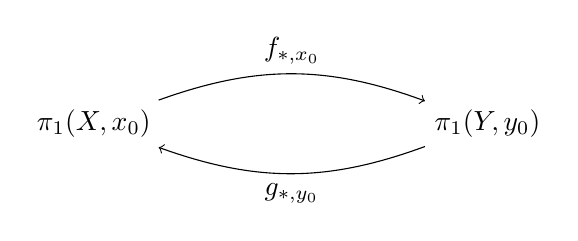
\begin{tikzpicture}
\node (A) at (0,0) {$\pi_1(X, x_0)$};
\node (B) at (5,0) {$\pi_1(Y, y_0)$};
\draw[->, bend left=20] (A) to node[above] {$f_{*,x_0}$} (B);
\draw[->, bend left=20] (B) to node[below] {$g_{*,y_0}$} (A);
\end{tikzpicture}
\end{center}
Por consiguiente, $f_{*,x_0}$ es un isomorfismo, con inversa $g_{*,y_0}$. Como $X$ e $Y$ son arco-conexos, $\pi_1(X) \cong \pi_1(X,x_0) \cong \pi_1(Y,y_0) \cong \pi_1(Y)$.
\end{proof}
\end{proposicion}

\begin{proposicion}{Grupo fundamental de un espacio estrellado [C6.5] \marcaE}{estrellado}
Sea $X \subseteq \mathbb{R}^n$, con $X$ estrellado. Entonces $\pi_1(X) = 1$.

\begin{proof}
Al ser estrellado, $X$ es arcoconexo (cada punto se une con el centro $x_0$ por un segmento), así que $\pi_1(X) = \pi_1(X, x_0) = C_{x_0}(X) / \simeq_{\{0,1\}}$. Además, existe un punto base $x_0 \in X$ tal que para todo $x \in X$ y todo $t \in [0,1]$, el segmento $t \cdot x + (1-t) \cdot x_0 \in X$.
Necesitamos probar que $[\alpha] = [c_{x_0}]$ para cualquier $\alpha \in C_{x_0}(X)$ (es decir, $\alpha \simeq_{\{0,1\}} c_{x_0}$).
Buscamos una homotopía $F \colon I \times I \longrightarrow X$ definida por:


$$F(s,t) = t \cdot \alpha(s) + (1-t) \cdot x_0$$


Comprobamos los extremos espaciales para asegurar que preserva el punto base:


$$F(0, t) = t \cdot \alpha(0) + (1-t) \cdot x_0 = t \cdot x_0 + (1-t) \cdot x_0 = x_0$$

$$F(1, t) = t \cdot \alpha(1) + (1-t) \cdot x_0 = t \cdot x_0 + (1-t) \cdot x_0 = x_0$$


Por tanto, $F$ es una homotopía de lazos que conecta el lazo constante $c_{x_0}$ (en $t=0$) con el lazo $\alpha$ (en $t=1$).
\end{proof}
\end{proposicion}

Los espacios estrellados son, por tanto, simplemente conexos (\cref{def:def_simp_conexo}). En particular, $\pi_1(I \times I) = 1$ y $\pi_1(\triangle) = 1$.

\subsection{Invariancia homotópica}

\begin{teorema}{Homomorfismos inducidos por aplicaciones homotópicas [C6.7] \marcaT}{aplicaciones_homotopicas}
Sean $f, g \colon X \to Y$ continuas, sea $F \colon f \simeq g$ una homotopía y sea $x_0 \in X$. Sea $\sigma \colon I \to Y$, $\sigma(t) = F(x_0, t)$, el arco que recorre el punto $x_0$ durante la homotopía, de $\sigma(0) = f(x_0)$ a $\sigma(1) = g(x_0)$. Consideramos:
\begin{itemize}
    \item $f_* \colon \pi_1(X,x_0) \to \pi_1(Y,f(x_0))$, $[\alpha] \mapsto [f \circ \alpha]$, y análogamente $g_*$;
    \item $P_\sigma \colon \pi_1(Y,f(x_0)) \to \pi_1(Y,g(x_0))$, $[\beta] \mapsto [\sigma^{-1} * \beta * \sigma]$, que es un isomorfismo (\cref{thm:teo_cambio_base}).
\end{itemize}
Entonces $g_* = P_\sigma \circ f_*$, es decir, el siguiente diagrama conmuta:
\begin{center}
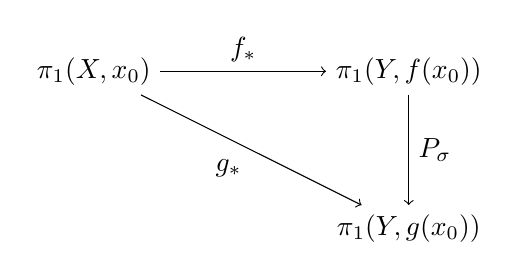
\begin{tikzpicture}
\node (A) at (0,2) {$\pi_1(X, x_0)$};
\node (B) at (4,2) {$\pi_1(Y, f(x_0))$};
\node (C) at (4,0) {$\pi_1(Y, g(x_0))$};
\draw[->] (A) -- (B) node[midway, above] {$f_*$};
\draw[->] (B) -- (C) node[midway, right] {$P_\sigma$};
\draw[->] (A) -- (C) node[midway, below left] {$g_*$};
\end{tikzpicture}
\end{center}

\begin{proof}
Para todo $[\alpha] \in \pi_1(X, x_0)$, necesitamos probar que $[g \circ \alpha] = [\sigma^{-1} * (f \circ \alpha) * \sigma]$.

Definimos $G \colon I \times I \longrightarrow Y$ por $G(s,t) = F(\alpha(s), t)$, que es continua (no es una homotopía relativa a los extremos). Tenemos $G_0 = f \circ \alpha$, $G_1 = g \circ \alpha$ y, como $\alpha(0) = \alpha(1) = x_0$,
\[ G(0,t) = G(1,t) = F(x_0,t) = \sigma(t) \quad \forall t \in I. \]

Recorremos el borde del cuadrado $I \times I$ con los cuatro arcos
\[ \lambda_1(s) = (0,s), \quad \lambda_2(s) = (s,1), \quad \lambda_3(s) = (1,1-s), \quad \lambda_4(s) = (1-s,0), \]
es decir, el lado izquierdo hacia arriba, el techo de izquierda a derecha, el lado derecho hacia abajo y la base de derecha a izquierda. Entonces $\gamma = \lambda_1 * \lambda_2 * \lambda_3 * \lambda_4$ es un lazo en $I \times I$ con base $(0,0)$.

\begin{center}
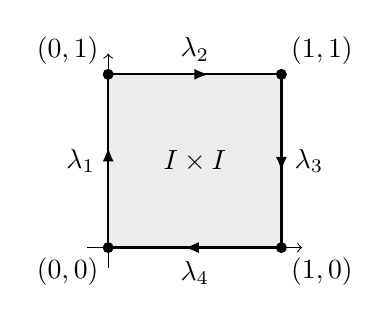
\begin{tikzpicture}[scale=2.2]
  \fill[gray!15] (0,0) rectangle (1,1);
  \draw[->] (0,-0.12) -- (0,1.12);
  \draw[->] (-0.12,0) -- (1.12,0);
  \draw[thick] (0,0) -- (0,1);
  \draw[thick] (0,1) -- (1,1);
  \draw[thick] (1,1) -- (1,0);
  \draw[thick] (1,0) -- (0,0);
  \draw[thick, -latex] (0,0.44) -- (0,0.58);
  \draw[thick, -latex] (0.44,1) -- (0.58,1);
  \draw[thick, -latex] (1,0.58) -- (1,0.44);
  \draw[thick, -latex] (0.58,0) -- (0.44,0);
  \filldraw (0,0) circle (0.8pt) node[below left] {$(0,0)$};
  \filldraw (1,0) circle (0.8pt) node[below right] {$(1,0)$};
  \filldraw (1,1) circle (0.8pt) node[above right] {$(1,1)$};
  \filldraw (0,1) circle (0.8pt) node[above left] {$(0,1)$};
  \node[left] at (-0.02,0.5) {$\lambda_1$};
  \node[above] at (0.5,1.02) {$\lambda_2$};
  \node[right] at (1.02,0.5) {$\lambda_3$};
  \node[below] at (0.5,-0.02) {$\lambda_4$};
  \node at (0.5,0.5) {$I \times I$};
\end{tikzpicture}
\end{center}

Calculamos las imágenes por $G$:
\begin{align*}
(G \circ \lambda_1)(s) &= G(0,s) = F(\alpha(0),s) = F(x_0,s) = \sigma(s), \\
(G \circ \lambda_2)(s) &= G(s,1) = F(\alpha(s),1) = (g \circ \alpha)(s), \\
(G \circ \lambda_3)(s) &= G(1,1-s) = F(x_0,1-s) = \sigma^{-1}(s), \\
(G \circ \lambda_4)(s) &= G(1-s,0) = F(\alpha(1-s),0) = (f \circ \alpha)(1-s),
\end{align*}
es decir, $G \circ \lambda_1 = \sigma$, $G \circ \lambda_2 = g \circ \alpha$, $G \circ \lambda_3 = \sigma^{-1}$ y $G \circ \lambda_4 = (f \circ \alpha)^{-1}$.
Como $G \circ (\lambda_1 * \dots * \lambda_4) = (G \circ \lambda_1) * \dots * (G \circ \lambda_4)$, se tiene
\[ G \circ \gamma = \sigma * (g \circ \alpha) * \sigma^{-1} * (f \circ \alpha)^{-1}, \]
que es un lazo en $Y$ con base $G(0,0) = f(x_0)$.

Como $I \times I$ es convexo, en particular estrellado, $\pi_1(I \times I) = 1$ (\cref{prop:estrellado}) y por tanto $\gamma \simeq_{\{0,1\}} c_{(0,0)}$. Componiendo esta homotopía con $G$ obtenemos $G \circ \gamma \simeq_{\{0,1\}} c_{f(x_0)}$, es decir,
\[ [\sigma] \cdot [g \circ \alpha] \cdot [\sigma^{-1}] \cdot [f \circ \alpha]^{-1} = [c_{f(x_0)}]. \]
Multiplicando por $[f \circ \alpha]$ por la derecha, $[\sigma] \cdot [g \circ \alpha] \cdot [\sigma^{-1}] = [f \circ \alpha]$, y multiplicando por $[\sigma^{-1}] = [\sigma]^{-1}$ por la izquierda y por $[\sigma]$ por la derecha obtenemos la relación buscada:
\[ [g \circ \alpha] = [\sigma^{-1}] \cdot [f \circ \alpha] \cdot [\sigma] = [\sigma^{-1} * (f \circ \alpha) * \sigma] \]
\end{proof}


\end{teorema}

\begin{nota}{Nota explicativa: el cuadrado enrollado}{nota_expl_homotopicas}
\begin{center}
\begin{tikzpicture}[scale=0.85, every node/.style={font=\small},
  marca/.style={postaction={decorate}, decoration={markings, mark=at position #1 with {\arrow{Stealth[length=5pt]}}}}]
\colorlet{cF}{blue!75!black}\colorlet{cG}{red!75!black}\colorlet{cS}{green!50!black}
\fill[gray!8] (0.00,0.40) rectangle (2.40,2.80);
\draw[cF, very thick, marca=0.55] (2.40,0.40) -- (0.00,0.40);
\draw[cG, very thick, marca=0.55] (0.00,2.80) -- (2.40,2.80);
\draw[cS, very thick, marca=0.6] (0.00,0.40) -- (0.00,2.80);
\draw[cS, very thick, marca=0.6] (2.40,2.80) -- (2.40,0.40);
\node[cF, below] at (1.20,0.40) {$\lambda_4$};
\node[cG, above] at (1.20,2.80) {$\lambda_2$};
\node[cS, left] at (0.00,1.60) {$\lambda_1$};
\node[cS, right] at (2.40,1.60) {$\lambda_3$};
\node at (1.20,1.60) {$I\times I$};
\draw[gray!60!black, -{Stealth[length=4pt]}] (0.00,-0.15) -- node[below, font=\scriptsize] {$s$} (0.70,-0.15);
\draw[gray!60!black, -{Stealth[length=4pt]}] (-0.70,0.40) -- node[left, font=\scriptsize] {$t$} (-0.70,1.10);
\draw[gray!60!black, fill=gray!8, fill opacity=0.6] (4.50,0.00) -- (7.90,0.00) -- (9.00,0.75) -- (5.60,0.75) -- cycle;
\node[gray!60!black, font=\scriptsize, anchor=west] at (8.45,0.38) {$X\times\{0\}$};
\draw[gray!60!black, fill=gray!8, fill opacity=0.6] (4.50,2.60) -- (7.90,2.60) -- (9.00,3.35) -- (5.60,3.35) -- cycle;
\node[gray!60!black, font=\scriptsize, anchor=west] at (8.45,2.98) {$X\times\{1\}$};
\draw[gray!60!black] (5.92,0.46) -- (5.92,3.06);
\draw[gray!60!black] (7.58,0.29) -- (7.58,2.89);
\draw[cF, very thick, dashed] plot coordinates {(7.58,0.29) (7.64,0.31) (7.68,0.33) (7.72,0.36) (7.76,0.38) (7.79,0.40) (7.81,0.43) (7.82,0.45) (7.83,0.47) (7.83,0.49) (7.83,0.52) (7.82,0.54) (7.80,0.56) (7.78,0.57) (7.75,0.59) (7.71,0.61) (7.67,0.62) (7.62,0.63) (7.57,0.64) (7.51,0.65) (7.44,0.66) (7.38,0.67) (7.31,0.67) (7.23,0.67) (7.15,0.67) (7.07,0.67) (6.99,0.67) (6.91,0.67) (6.82,0.66) (6.74,0.65) (6.65,0.64) (6.57,0.63) (6.48,0.61) (6.40,0.60) (6.32,0.58) (6.25,0.57) (6.17,0.55) (6.10,0.53) (6.04,0.51) (5.97,0.48) (5.92,0.46)};
\draw[cF, very thick, marca=0.75] plot coordinates {(5.92,0.46) (5.86,0.44) (5.82,0.42) (5.78,0.39) (5.74,0.37) (5.71,0.35) (5.69,0.32) (5.68,0.30) (5.67,0.28) (5.67,0.26) (5.67,0.23) (5.68,0.21) (5.70,0.19) (5.72,0.18) (5.75,0.16) (5.79,0.14) (5.83,0.13) (5.88,0.12) (5.93,0.11) (5.99,0.10) (6.06,0.09) (6.12,0.08) (6.19,0.08) (6.27,0.08) (6.35,0.08) (6.43,0.08) (6.51,0.08) (6.59,0.08) (6.68,0.09) (6.76,0.10) (6.85,0.11) (6.93,0.12) (7.02,0.14) (7.10,0.15) (7.18,0.17) (7.25,0.18) (7.33,0.20) (7.40,0.22) (7.46,0.24) (7.53,0.27) (7.58,0.29)};
\draw[cG, very thick, marca=0.3] plot coordinates {(7.75,2.98) (7.80,3.02) (7.83,3.07) (7.83,3.11) (7.81,3.15) (7.76,3.18) (7.69,3.21) (7.60,3.24) (7.48,3.26) (7.35,3.27) (7.21,3.27) (7.05,3.27) (6.89,3.26) (6.73,3.25) (6.56,3.23) (6.40,3.20) (6.25,3.17) (6.11,3.13) (5.98,3.09) (5.87,3.04) (5.79,3.00) (5.72,2.95) (5.68,2.91) (5.67,2.86) (5.68,2.82) (5.71,2.79) (5.77,2.75) (5.85,2.72) (5.95,2.70) (6.08,2.69) (6.21,2.68) (6.36,2.68) (6.52,2.68) (6.69,2.69) (6.85,2.71) (7.02,2.74) (7.17,2.77) (7.32,2.80) (7.45,2.84) (7.57,2.88) (7.67,2.93)} -- cycle;
\draw[cS, very thick, marca=0.6] (5.69,0.20) -- (5.69,2.80);
\fill[cS] (5.69,0.20) circle (1.7pt); \fill[cS] (5.69,2.80) circle (1.7pt);
\node[cS, font=\scriptsize, anchor=west] at (5.77,1.50) {$\{x_0\}\times I$};
\node[cF, font=\scriptsize] at (7.00,-0.22) {$\alpha\times\{0\}$};
\node[cG, font=\scriptsize] at (7.00,3.58) {$\alpha\times\{1\}$};
\draw[orange!70!black, fill=orange!6, thick] plot[smooth cycle, tension=0.8] coordinates {(3.82,-3.70) (4.68,-5.24) (6.95,-5.59) (9.65,-5.18) (11.38,-3.82) (11.16,-2.05) (9.11,-1.29) (6.30,-1.40) (4.25,-2.23)};
\node[orange!70!black] at (4.30,-1.75) {$Y$};
\draw[gray!50, thin] plot[smooth, tension=0.7] coordinates {(5.41,-2.40) (7.68,-2.50) (10.02,-2.10)};
\draw[gray!50, thin] plot[smooth, tension=0.7] coordinates {(5.19,-4.50) (7.51,-4.20) (9.79,-4.40)};
\draw[cF, very thick, dashed, opacity=0.55] plot coordinates {(5.41,-2.40) (5.37,-2.42) (5.33,-2.45) (5.30,-2.48) (5.26,-2.52) (5.23,-2.56) (5.20,-2.61) (5.16,-2.66) (5.13,-2.72) (5.10,-2.78) (5.08,-2.85) (5.05,-2.92) (5.02,-2.99) (5.00,-3.07) (4.97,-3.15) (4.95,-3.23) (4.93,-3.32) (4.91,-3.41) (4.90,-3.50) (4.89,-3.59) (4.88,-3.68) (4.87,-3.78) (4.87,-3.87) (4.87,-3.96) (4.88,-4.05) (4.89,-4.13) (4.90,-4.20) (4.92,-4.27) (4.94,-4.33) (4.97,-4.39) (4.99,-4.43) (5.02,-4.47) (5.06,-4.49) (5.09,-4.51) (5.12,-4.51) (5.16,-4.51) (5.19,-4.50)};
\draw[cF, very thick, marca=0.5] plot coordinates {(5.19,-4.50) (5.23,-4.48) (5.27,-4.45) (5.30,-4.42) (5.34,-4.38) (5.37,-4.34) (5.40,-4.29) (5.44,-4.24) (5.47,-4.18) (5.50,-4.12) (5.52,-4.05) (5.55,-3.98) (5.58,-3.91) (5.60,-3.83) (5.63,-3.75) (5.65,-3.67) (5.67,-3.58) (5.69,-3.49) (5.70,-3.40) (5.71,-3.31) (5.72,-3.22) (5.73,-3.12) (5.73,-3.03) (5.73,-2.94) (5.72,-2.85) (5.71,-2.77) (5.70,-2.70) (5.68,-2.63) (5.66,-2.57) (5.63,-2.51) (5.61,-2.47) (5.58,-2.43) (5.54,-2.41) (5.51,-2.39) (5.48,-2.39) (5.44,-2.39) (5.41,-2.40)};
\draw[violet!55, thick, dashed, opacity=0.55] plot coordinates {(7.68,-2.50) (7.65,-2.51) (7.62,-2.52) (7.59,-2.54) (7.56,-2.57) (7.52,-2.60) (7.49,-2.64) (7.46,-2.68) (7.43,-2.73) (7.41,-2.78) (7.38,-2.84) (7.35,-2.90) (7.33,-2.96) (7.31,-3.03) (7.29,-3.10) (7.27,-3.17) (7.26,-3.24) (7.25,-3.32) (7.24,-3.39) (7.23,-3.47) (7.23,-3.54) (7.23,-3.61) (7.23,-3.68) (7.24,-3.75) (7.25,-3.81) (7.26,-3.87) (7.27,-3.93) (7.29,-3.98) (7.30,-4.03) (7.32,-4.07) (7.35,-4.11) (7.37,-4.14) (7.40,-4.16) (7.42,-4.18) (7.45,-4.19) (7.48,-4.20) (7.51,-4.20)};
\draw[violet!55, thick] plot coordinates {(7.51,-4.20) (7.55,-4.19) (7.58,-4.18) (7.61,-4.16) (7.64,-4.13) (7.68,-4.10) (7.71,-4.06) (7.74,-4.02) (7.77,-3.97) (7.79,-3.92) (7.82,-3.86) (7.85,-3.80) (7.87,-3.74) (7.89,-3.67) (7.91,-3.60) (7.93,-3.53) (7.94,-3.46) (7.95,-3.38) (7.96,-3.31) (7.97,-3.23) (7.97,-3.16) (7.97,-3.09) (7.97,-3.02) (7.96,-2.95) (7.95,-2.89) (7.94,-2.83) (7.93,-2.77) (7.91,-2.72) (7.90,-2.67) (7.88,-2.63) (7.85,-2.59) (7.83,-2.56) (7.80,-2.54) (7.78,-2.52) (7.75,-2.51) (7.72,-2.50) (7.68,-2.50)};
\draw[cG, very thick, dashed, opacity=0.55] plot coordinates {(10.02,-2.10) (9.98,-2.10) (9.94,-2.10) (9.90,-2.12) (9.86,-2.15) (9.82,-2.18) (9.78,-2.23) (9.75,-2.29) (9.71,-2.35) (9.67,-2.43) (9.64,-2.51) (9.61,-2.60) (9.58,-2.69) (9.55,-2.79) (9.53,-2.89) (9.51,-2.99) (9.50,-3.10) (9.49,-3.20) (9.48,-3.30) (9.48,-3.40) (9.48,-3.49) (9.48,-3.59) (9.48,-3.67) (9.49,-3.76) (9.50,-3.84) (9.51,-3.91) (9.53,-3.98) (9.54,-4.05) (9.56,-4.11) (9.58,-4.17) (9.61,-4.22) (9.63,-4.26) (9.66,-4.31) (9.69,-4.34) (9.72,-4.37) (9.75,-4.39) (9.79,-4.40)};
\draw[cG, very thick, marca=0.5] plot coordinates {(9.79,-4.40) (9.82,-4.40) (9.86,-4.40) (9.90,-4.38) (9.94,-4.35) (9.98,-4.32) (10.02,-4.27) (10.05,-4.21) (10.09,-4.15) (10.13,-4.07) (10.16,-3.99) (10.19,-3.90) (10.22,-3.81) (10.25,-3.71) (10.27,-3.61) (10.29,-3.51) (10.30,-3.40) (10.31,-3.30) (10.32,-3.20) (10.32,-3.10) (10.32,-3.01) (10.32,-2.91) (10.32,-2.83) (10.31,-2.74) (10.30,-2.66) (10.29,-2.59) (10.27,-2.52) (10.26,-2.45) (10.24,-2.39) (10.22,-2.33) (10.19,-2.28) (10.17,-2.24) (10.14,-2.19) (10.11,-2.16) (10.08,-2.13) (10.05,-2.11) (10.02,-2.10)};
\draw[cS, very thick, -{Stealth[length=6pt]}] plot[smooth, tension=0.7] coordinates {(5.09,-4.51) (7.42,-4.30) (9.69,-4.34)};
\draw[cS, thick, dashed, -{Stealth[length=6pt]}] plot[smooth, tension=0.7] coordinates {(9.64,-4.56) (7.42,-4.68) (5.14,-4.73)};
\fill[cF] (5.09,-4.51) circle (1.8pt); \fill[cG] (9.69,-4.34) circle (1.8pt);
\node[cF, anchor=east, font=\scriptsize, inner sep=2pt] at (5.01,-4.51) {$f(x_0)$};
\node[cG, anchor=north west, font=\scriptsize, inner sep=1pt] at (9.74,-4.39) {$g(x_0)$};
\node[cS, font=\scriptsize, fill=orange!6, inner sep=1pt] at (8.32,-4.13) {$\sigma$};
\node[cS, font=\scriptsize, fill=orange!6, inner sep=1pt] at (8.32,-4.78) {$\sigma^{-1}$};
\node[cF, font=\scriptsize] at (5.30,-2.15) {$f\circ\alpha$};
\node[cG, font=\scriptsize] at (9.90,-1.85) {$g\circ\alpha$};
\node[violet!70!black, font=\scriptsize] at (7.60,-2.25) {$F_t\circ\alpha$};
\draw[gray!60!black, thick, -{Stealth[length=6pt]}] (3.05,1.75) to[bend left=18] node[above=2pt, font=\scriptsize] {$(s,t)\mapsto(\alpha(s),t)$} (4.55,1.45);
\draw[gray!60!black, thick, -{Stealth[length=6pt]}] (9.3,-0.15) to[bend left=25] node[right] {$F$} (9.6,-1.2);
\end{tikzpicture}
\end{center}
El cuadrado se \emph{enrolla} en el cilindro $\alpha \times I \subseteq X \times I$: la base y el techo se cierran en los lazos $\alpha \times \{0\}$ y $\alpha \times \{1\}$, y los lados $\lambda_1$, $\lambda_3$ se pegan en el segmento $\{x_0\} \times I$. Después $F$ lo lleva a $Y$: la base da $f \circ \alpha$, el techo $g \circ \alpha$, y la costura da $\sigma$ (recorrida a la ida por $\lambda_1$ y a la vuelta, como $\sigma^{-1}$, por $\lambda_3$). Como el cuadrado se contrae, su borde ($\sigma$, $g \circ \alpha$, $\sigma^{-1}$, $(f \circ \alpha)^{-1}$) es trivial en $Y$, y eso es $g_* = P_\sigma \circ f_*$: $g$ actúa sobre los lazos igual que $f$, pero vista desde el punto base desplazado por $\sigma$.

\textbf{Atajo.} En el convexo $I\times I$, los caminos $\lambda_2$ (por arriba) y $\delta=\lambda_1^{-1}*\lambda_4^{-1}*\lambda_3^{-1}$ (por abajo) van de $(0,1)$ a $(1,1)$, luego $\lambda_2\simeq_{\{0,1\}}\delta$ por la homotopía recta; componiendo con $G$ sale directamente $g\circ\alpha\simeq_{\{0,1\}}\sigma^{-1}*(f\circ\alpha)*\sigma$, sin despejar en el grupo.
\end{nota}


\begin{proposicion}{Equivalencia Homotópica [C6.8] \marcaC}{equiv_homotopica}
Sean $X, Y$ espacios arco-conexos. Si $X$ e $Y$ tienen el mismo tipo de homotopía ($X \simeq Y$), entonces $\pi_1(X) \cong \pi_1(Y)$.

\begin{proof}
Sean $f \colon X \to Y$ y $g \colon Y \to X$ continuas con $g \circ f \simeq 1_X$ y $f \circ g \simeq 1_Y$. Sea $x_0 \in X$ e $y_0 = f(x_0)$.
\begin{align*}
    &1.\; F \colon 1_X \simeq g \circ f, \quad \sigma(t) = F(x_0,t) \\
    &\qquad \Longrightarrow (g \circ f)_{*,x_0} = P_\sigma \circ (1_X)_{*,x_0} = P_\sigma, \text{ isomorfismo (\cref{thm:aplicaciones_homotopicas}).} \\
    &2.\; (g \circ f)_{*,x_0} = g_{*,y_0} \circ f_{*,x_0} \text{ biyectiva} \\
    &\qquad \Longrightarrow f_{*,x_0} \text{ inyectiva y } g_{*,y_0} \textbf{ sobreyectiva}. \\
    &3.\; G \colon 1_Y \simeq f \circ g, \quad \tau(t) = G(y_0,t) \\
    &\qquad \Longrightarrow (f \circ g)_{*,y_0} = P_\tau, \text{ isomorfismo}. \\
    &4.\; (f \circ g)_{*,y_0} = f_{*,g(y_0)} \circ g_{*,y_0} \text{ biyectiva} \\
    &\qquad \Longrightarrow g_{*,y_0} \textbf{ inyectiva} \text{ (y } f_{*,g(y_0)} \text{ sobreyectiva)}. \\
    &\text{De 2 y 4:} \\
    &\qquad \Longrightarrow g_{*,y_0} \colon \pi_1(Y,y_0) \to \pi_1(X,g(y_0)) \text{ es isomorfismo} \\
    &\qquad \Longrightarrow \pi_1(Y) \cong \pi_1(X), \text{ por ser arco-conexos.}
\end{align*}
\end{proof}
\end{proposicion}


\begin{observacion}{Invariancia homotópica vs. invariancia topológica [C6.8]}{obs_invariancia_homotopica}
La proposición anterior es más general que la invariancia topológica del grupo fundamental (homeomorfismo induce isomorfismo): como $X \cong Y \implies X \simeq Y$, esta última es un caso particular. La inclusión es estricta: por ejemplo $D(0,1) \simeq \{\text{punto}\}$ sin ser homeomorfos, y la invariancia homotópica da $\pi_1(D(0,1)) \cong \pi_1(\{\text{punto}\}) = 1$, algo que la invariancia topológica no permite deducir. Igualmente, $S^1 \times [-1,1] \simeq S^1$ y por tanto ambos tienen el mismo grupo fundamental aunque no sean homeomorfos.
\end{observacion}